\documentclass[12pt,]{article}
\usepackage{lmodern}
\usepackage{amssymb,amsmath}
\usepackage{ifxetex,ifluatex}
\usepackage{fixltx2e} % provides \textsubscript
\ifnum 0\ifxetex 1\fi\ifluatex 1\fi=0 % if pdftex
  \usepackage[T1]{fontenc}
  \usepackage[utf8]{inputenc}
\else % if luatex or xelatex
  \ifxetex
    \usepackage{mathspec}
  \else
    \usepackage{fontspec}
  \fi
  \defaultfontfeatures{Ligatures=TeX,Scale=MatchLowercase}
    \setmainfont[]{Times New Roman}
\fi
% use upquote if available, for straight quotes in verbatim environments
\IfFileExists{upquote.sty}{\usepackage{upquote}}{}
% use microtype if available
\IfFileExists{microtype.sty}{%
\usepackage{microtype}
\UseMicrotypeSet[protrusion]{basicmath} % disable protrusion for tt fonts
}{}
\usepackage[margin=1in]{geometry}
\usepackage{hyperref}
\PassOptionsToPackage{usenames,dvipsnames}{color} % color is loaded by hyperref
\hypersetup{unicode=true,
            pdftitle={PROJECT REPORT},
            pdfauthor={Diane Kamning},
            colorlinks=true,
            linkcolor=Maroon,
            citecolor=Blue,
            urlcolor=blue,
            breaklinks=true}
\urlstyle{same}  % don't use monospace font for urls
\usepackage{longtable,booktabs}
\usepackage{graphicx,grffile}
\makeatletter
\def\maxwidth{\ifdim\Gin@nat@width>\linewidth\linewidth\else\Gin@nat@width\fi}
\def\maxheight{\ifdim\Gin@nat@height>\textheight\textheight\else\Gin@nat@height\fi}
\makeatother
% Scale images if necessary, so that they will not overflow the page
% margins by default, and it is still possible to overwrite the defaults
% using explicit options in \includegraphics[width, height, ...]{}
\setkeys{Gin}{width=\maxwidth,height=\maxheight,keepaspectratio}
\IfFileExists{parskip.sty}{%
\usepackage{parskip}
}{% else
\setlength{\parindent}{0pt}
\setlength{\parskip}{6pt plus 2pt minus 1pt}
}
\setlength{\emergencystretch}{3em}  % prevent overfull lines
\providecommand{\tightlist}{%
  \setlength{\itemsep}{0pt}\setlength{\parskip}{0pt}}
\setcounter{secnumdepth}{5}
% Redefines (sub)paragraphs to behave more like sections
\ifx\paragraph\undefined\else
\let\oldparagraph\paragraph
\renewcommand{\paragraph}[1]{\oldparagraph{#1}\mbox{}}
\fi
\ifx\subparagraph\undefined\else
\let\oldsubparagraph\subparagraph
\renewcommand{\subparagraph}[1]{\oldsubparagraph{#1}\mbox{}}
\fi

%%% Use protect on footnotes to avoid problems with footnotes in titles
\let\rmarkdownfootnote\footnote%
\def\footnote{\protect\rmarkdownfootnote}

%%% Change title format to be more compact
\usepackage{titling}

% Create subtitle command for use in maketitle
\newcommand{\subtitle}[1]{
  \posttitle{
    \begin{center}\large#1\end{center}
    }
}

\setlength{\droptitle}{-2em}
  \title{PROJECT REPORT}
  \pretitle{\vspace{\droptitle}\centering\huge}
  \posttitle{\par}
\subtitle{FINANCIAL TRADING STRATEGY}
  \author{Diane Kamning}
  \preauthor{\centering\large\emph}
  \postauthor{\par}
  \predate{\centering\large\emph}
  \postdate{\par}
  \date{March 22, 2017}

\setlength\parindent{24pt}

\begin{document}
\maketitle

{
\hypersetup{linkcolor=black}
\setcounter{tocdepth}{2}
\tableofcontents
}
\pagebreak

\section{INTRODUCTION}\label{introduction}

This project aims at building a model that will ideally always output
successful bids in the stock market. For that, it builds a model which
gives better results when constantly trained in a sliding-time window.
The goal is to design a simple financial trading strategy that will be
profitable and that will provide a good risk-adjusted measure of return.

\section{DATA SETS}\label{data-sets}

Two datasets will be used here to test the strategy:

\begin{itemize}
\tightlist
\item
  The American Electric Company (AEP) dataset from Quandl
\end{itemize}

\begin{longtable}[]{@{}rrrrrr@{}}
\toprule
Open & High & Low & Close & Volume & Ex-Dividend\tabularnewline
\midrule
\endhead
32.00 & 32.00 & 31.12 & 31.44 & 396900 & 0\tabularnewline
31.38 & 31.94 & 31.38 & 31.81 & 325500 & 0\tabularnewline
31.94 & 33.13 & 31.88 & 33.00 & 392200 & 0\tabularnewline
32.75 & 33.69 & 32.75 & 33.19 & 433000 & 0\tabularnewline
33.38 & 33.75 & 33.06 & 33.63 & 250500 & 0\tabularnewline
33.63 & 33.81 & 33.44 & 33.50 & 307700 & 0\tabularnewline
\bottomrule
\end{longtable}

\begin{itemize}
\tightlist
\item
  The Chesapeake Energy Corporation (CHK) from Quandl.
\end{itemize}

\begin{longtable}[]{@{}rrrrrr@{}}
\toprule
Open & High & Low & Close & Volume & Ex-Dividend\tabularnewline
\midrule
\endhead
2.31 & 2.38 & 2.25 & 2.25 & 369700 & 0\tabularnewline
2.19 & 2.25 & 2.06 & 2.06 & 719400 & 0\tabularnewline
2.12 & 2.19 & 1.94 & 2.06 & 807100 & 0\tabularnewline
1.94 & 2.12 & 1.94 & 2.12 & 444900 & 0\tabularnewline
2.06 & 2.12 & 2.06 & 2.06 & 207400 & 0\tabularnewline
2.06 & 2.12 & 2.06 & 2.12 & 166700 & 0\tabularnewline
\bottomrule
\end{longtable}

An initial exploration of the AEP dataset reveals 5 important fields:

\begin{itemize}
\tightlist
\item
  The date
\item
  The Open price
\item
  The High price
\item
  The Low price
\item
  The Close price.
\end{itemize}

Some of the issues encountered with the data:

\begin{itemize}
\tightlist
\item
  The presence of the adjusted closing price was confusing for some
  methods in the packages Quandstrat and xts, as those methods kept
  throwing errors. I had to remove the adjusted closing price from my
  data sets and just keep the closing price
\item
  Some functions and arguments were not found because the Quandstrat
  package is not yet stable.
\end{itemize}

\section{PRELIMINARY EXPLORATION}\label{preliminary-exploration}

Indicators are transformations of market data that give an insight into
the overall market behavior by measuring current conditions and/or
forecasting trends. Among others, there are trend-following indicators
which depict the general price direction, and oscillators used to
discover on a scale of 0 to 100 short-term overbought (above 70 to 80)
or oversold (below 30 to 20) conditions . Combining trend-following
indicators and oscillator/reversion indicators gives more insight into
the data for this project. The preliminary oscillator used is an RSI
(Relative Strength Index) with a 3-days lookback period. The preliminary
trend indicators are 3 SMA (Simple Moving Average). After applying those
indicators to the stocks, there are some periods of time during which
none of the indicators seem to be right.

\subsection{TREND-FOLLOWING INDICATORS: SIMPLE MOVING
AVERAGES}\label{trend-following-indicators-simple-moving-averages}

The SMA50 (Simple Moving Average) seems to better mimic the trend of the
closing prices for both data sets

\begin{itemize}
\tightlist
\item
  SMA AEP
\end{itemize}

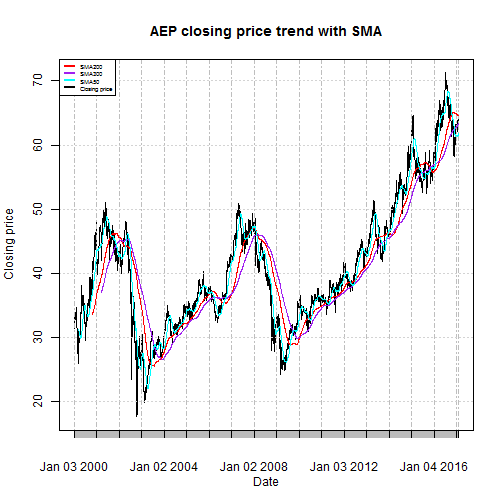
\includegraphics{ProjectReport_files/figure-latex/unnamed-chunk-4-1.pdf}

\begin{itemize}
\tightlist
\item
  SMA CHK
\end{itemize}

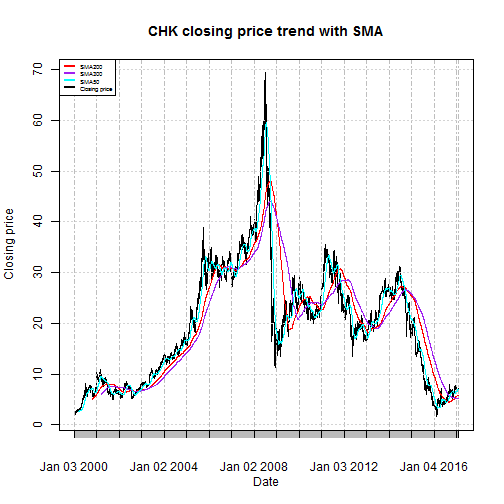
\includegraphics{ProjectReport_files/figure-latex/unnamed-chunk-5-1.pdf}

\subsection{OSCILLATOR/REVERSION INDICATOR:
RSI}\label{oscillatorreversion-indicator-rsi}

An observation of the graphs of the stocks’ RSI reveals that there are
effectively periods of reversion (2013-09-03 to 2013-9-05 for example)
that won’t be captured by a trend-following indicator:

\begin{itemize}
\tightlist
\item
  RSI AEP
\end{itemize}

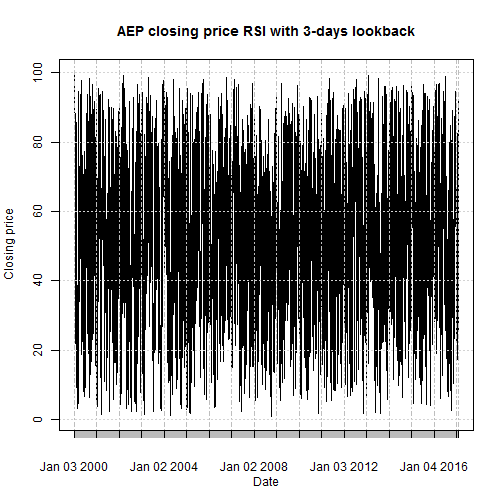
\includegraphics{ProjectReport_files/figure-latex/unnamed-chunk-6-1.pdf}

\begin{itemize}
\tightlist
\item
  RSI CHK
\end{itemize}

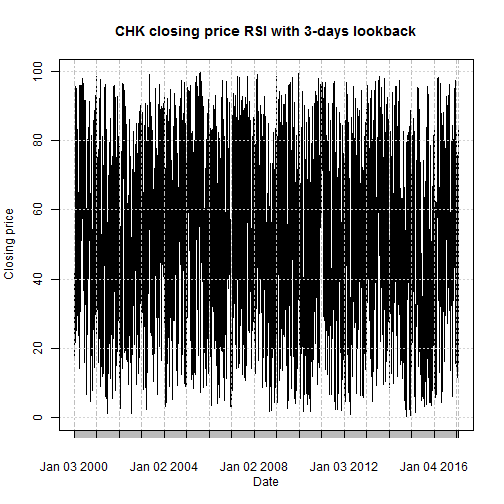
\includegraphics{ProjectReport_files/figure-latex/unnamed-chunk-7-1.pdf}

\section{APPROACH}\label{approach}

The main objective is to obtain a profit factor (monetary unit gained
per monetary unit lost) above 1 after running the strategy on each of
the data sets. The approach here would be to combine both SMA50 and
SMA200 with an oscillator to avoid false signals. The trend-following
indicators would help catch up trends.\\
The analysis is done on 16 years, from January 01st, 2000 to December
31st, 2016 . The time is Eastern time and the currency is US dollar.

\subsection{STRATEGY 1: RSI}\label{strategy-1-rsi}

``RSI Strategy'', the initial strategy for this project, uses simple
averages (over 50 days and over 200 days) with a custom RSI\_3\_4
indicator acting as an average between RSI3 and RSI4 . Signals help
interpret how indicators interact with the market and with each other.
Those signals are:

\begin{itemize}
\tightlist
\item
  a comparison and a crossover , which show a buy signal when the 50-day
  simple moving average is above the 200-day simple moving average and
  show a sell signal when the 50-day simple moving average crosses below
  the 200-day simple moving average
\item
  a threshold, which an oversold condition, thus a buy opportunity, for
  RSI\_3\_4 below 20, and an overbought condition, thus a sell
  opportunity, for RSI\_3\_4 above 80
\item
  a combined comparison and threshold to buy when the 50-day simple
  moving average is above the 200-day simple moving average and
  RSI\_3\_4 is less than 20.
\end{itemize}

\begin{verbatim}
## 
## 
## Table: AEP Subset
## 
##                    2013-09-03   2013-09-04   2013-09-05
## ----------------  -----------  -----------  -----------
## Open                 43.03000     42.16000     42.19000
## High                 43.13000     42.34000     42.45000
## Low                  42.07000     41.83000     42.07000
## Close                42.16000     42.21000     42.14000
## SMA.SMA200           45.75490     45.76115     45.76425
## SMA.SMA50            44.93140     44.90420     44.86880
## RSI_avg.RSI_3_4      22.85453     26.99133     24.42352
## longfilter            0.00000      0.00000      0.00000
## filterexit                 NA           NA           NA
## longthreshold         0.00000      0.00000      0.00000
## thresholdexit         0.00000      0.00000      0.00000
## longentry             0.00000      0.00000      0.00000
\end{verbatim}

\begin{verbatim}
## 
## 
## Table: CHK Subset
## 
##                    2013-09-03   2013-09-04   2013-09-05
## ----------------  -----------  -----------  -----------
## Open                 26.07000     26.09000     26.18000
## High                 26.41000     26.18000     26.24000
## Low                  26.02000     26.00000     26.02000
## Close                26.16000     26.12000     26.17000
## SMA.SMA200           20.35310     20.40175     20.44950
## SMA.SMA50            23.32000     23.45040     23.57800
## RSI_avg.RSI_3_4      61.91683     58.61329     62.21049
## longfilter            1.00000      1.00000      1.00000
## filterexit                 NA           NA           NA
## longthreshold         0.00000      0.00000      0.00000
## thresholdexit         0.00000      0.00000      0.00000
## longentry             0.00000      0.00000      0.00000
\end{verbatim}

Rules help shape trading transactions at signal execution. They generate
orders using market data, indicators and signals. This strategy has 2
rules:

\begin{itemize}
\tightlist
\item
  an entry rule of 1 share for the combined comparison and threshold
  entry signals
\item
  an exit rule for a treshold above 80.
\end{itemize}

Running this RSI\_3\_4 strategy on the AEP and the CHK over that trading
period, yields profit factors above 1, meaning that the strategy is
profitable:

\begin{longtable}[]{@{}llr@{}}
\toprule
& Symbol & Profit.Factor\tabularnewline
\midrule
\endhead
stockAEP & stockAEP & 1.952576\tabularnewline
stockCHK & stockCHK & 1.463076\tabularnewline
\bottomrule
\end{longtable}

Let's take a look at the system performance for the 2 stocks:

\begin{itemize}
\tightlist
\item
  Stock 1: AEP
\end{itemize}

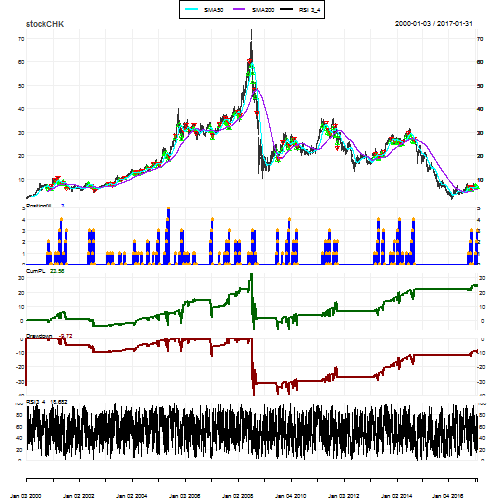
\includegraphics{ProjectReport_files/figure-latex/unnamed-chunk-15-1.pdf}

\begin{itemize}
\tightlist
\item
  stock 2: CHK
\end{itemize}

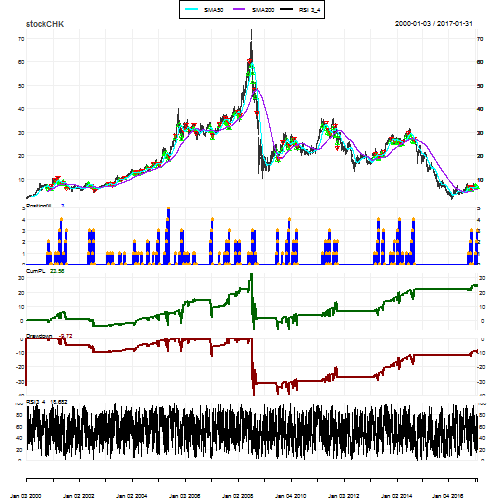
\includegraphics{ProjectReport_files/figure-latex/unnamed-chunk-16-1.pdf}

We can further analyze this RSI-3\_4 strategy by getting the order book
and retrieving the trade statistics:

\begin{longtable}[]{@{}lll@{}}
\toprule
& stockAEP & stockCHK\tabularnewline
\midrule
\endhead
Portfolio & RSI strategy & RSI strategy\tabularnewline
Symbol & stockAEP & stockCHK\tabularnewline
Num.Txns & 169 & 177\tabularnewline
Num.Trades & 55 & 58\tabularnewline
Net.Trading.PL & 37.16 & 23.56\tabularnewline
Avg.Trade.PL & 0.6756364 & 0.4194828\tabularnewline
Med.Trade.PL & 1.05 & 1.13\tabularnewline
Largest.Winner & 7.92 & 5.86\tabularnewline
Largest.Loser & -9.42 & -19.36\tabularnewline
Gross.Profits & 76.17 & 76.87\tabularnewline
Gross.Losses & -39.01 & -52.54\tabularnewline
Std.Dev.Trade.PL & 2.915206 & 3.585156\tabularnewline
Percent.Positive & 70.90909 & 75.86207\tabularnewline
Percent.Negative & 29.09091 & 24.13793\tabularnewline
Profit.Factor & 1.952576 & 1.463076\tabularnewline
Avg.Win.Trade & 1.953077 & 1.747045\tabularnewline
Med.Win.Trade & 1.500 & 1.485\tabularnewline
Avg.Losing.Trade & -2.438125 & -3.752857\tabularnewline
Med.Losing.Trade & -1.15 & -1.97\tabularnewline
Avg.Daily.PL & 0.6756364 & 0.4194828\tabularnewline
Med.Daily.PL & 1.05 & 1.13\tabularnewline
Std.Dev.Daily.PL & 2.915206 & 3.585156\tabularnewline
Ann.Sharpe & 3.679120 & 1.857404\tabularnewline
Max.Drawdown & -24.44 & -39.85\tabularnewline
Profit.To.Max.Draw & 1.5204583 & 0.5912171\tabularnewline
Avg.WinLoss.Ratio & 0.8010569 & 0.4655241\tabularnewline
Med.WinLoss.Ratio & 1.3043478 & 0.7538071\tabularnewline
Max.Equity & 38.81 & 33.28\tabularnewline
Min.Equity & -4.56 & -6.57\tabularnewline
End.Equity & 37.16 & 23.56\tabularnewline
\bottomrule
\end{longtable}

\begin{longtable}[]{@{}lrr@{}}
\toprule
& stockAEP.DailyEndEq & stockCHK.DailyEndEq\tabularnewline
\midrule
\endhead
Annualized Sharpe Ratio (Rf=0\%) & 0.1945513 & 0.1296419\tabularnewline
\bottomrule
\end{longtable}

For both instruments, the profit factor (absolute value ratio of gross
profits over gross losses ) is above 1 . Therefore, this strategy is
profitable.

\[Profit factor = Abs( gross profits / gross losses)\]

The Sharpe Ratio is a risk-adjusted measure of return.

\[ Sharpe ratio = (Mean portfolio return - Risk-free rate ) / Standard deviation of portfolio return \]

With the Quandstart R package, there are ways to get the cash Sharpe
Ratio (Sharpe Ratio from profit and loss) and the returns-based Sharpe
Ratio (Sharpe Ratio from P\&L over initial equity) of a strategy. The
annualized returns-based Sharpe Ratios are low, the highest being
\textasciitilde{} 0.23 on stock AEP. Let's try to increase the
annualized returns-based Sharpe ratio by changing the oscillator of this
strategy.

\subsection{STRATEGY 2: DVO}\label{strategy-2-dvo}

Instead of using the RSI\_3\_4 as the oscillator, let's use a custom DVO
with navg = 2 and a percentlookback period of 126 that we call
DVO\_2\_126 . The trend following indicators SMA50 and SMA200 stay the
same , as well as the signals, rules and settings of the strategy.

\begin{verbatim}
## 
## 
## Table: AEP Subset
## 
##                  2013-09-03   2013-09-04   2013-09-05
## --------------  -----------  -----------  -----------
## Open              43.030000     42.16000     42.19000
## High              43.130000     42.34000     42.45000
## Low               42.070000     41.83000     42.07000
## Close             42.160000     42.21000     42.14000
## SMA.SMA200        45.754900     45.76115     45.76425
## SMA.SMA50         44.931400     44.90420     44.86880
## DVO.DVO_2_126      6.349206     15.87302     53.17460
## longfilter         0.000000      0.00000      0.00000
## filterexit               NA           NA           NA
## longthreshold      1.000000      1.00000      0.00000
## thresholdexit      0.000000      0.00000      0.00000
## longentry          0.000000      0.00000      0.00000
\end{verbatim}

\begin{verbatim}
## 
## 
## Table: CHK Subset
## 
##                  2013-09-03   2013-09-04   2013-09-05
## --------------  -----------  -----------  -----------
## Open               26.07000     26.09000      26.1800
## High               26.41000     26.18000      26.2400
## Low                26.02000     26.00000      26.0200
## Close              26.16000     26.12000      26.1700
## SMA.SMA200         20.35310     20.40175      20.4495
## SMA.SMA50          23.32000     23.45040      23.5780
## DVO.DVO_2_126      30.15873     40.47619      53.1746
## longfilter          1.00000      1.00000       1.0000
## filterexit               NA           NA           NA
## longthreshold       0.00000      0.00000       0.0000
## thresholdexit       0.00000      0.00000       0.0000
## longentry           0.00000      0.00000       0.0000
\end{verbatim}

Let's run the DVO strategy.

Performance of the systems:

\begin{itemize}
\tightlist
\item
  stock 1: AEP
\end{itemize}

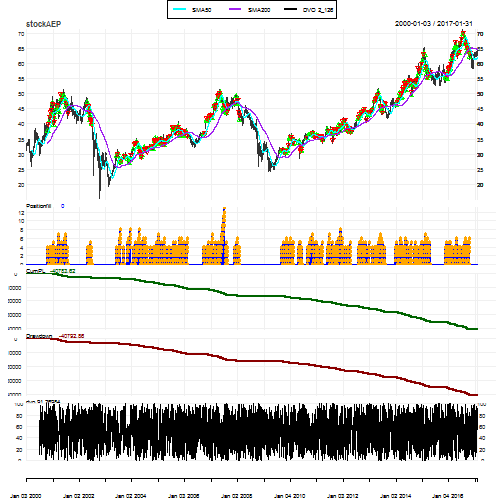
\includegraphics{ProjectReport_files/figure-latex/unnamed-chunk-24-1.pdf}

\begin{itemize}
\tightlist
\item
  stock 2: CHK
\end{itemize}

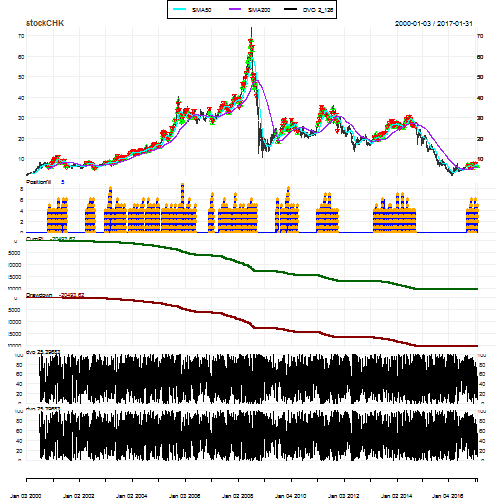
\includegraphics{ProjectReport_files/figure-latex/unnamed-chunk-25-1.pdf}

Analyzing this DVO strategy, we get the following trade metrics:

\begin{longtable}[]{@{}lll@{}}
\toprule
& stockAEP & stockCHK\tabularnewline
\midrule
\endhead
Portfolio & DVO strategy & DVO strategy\tabularnewline
Symbol & stockAEP & stockCHK\tabularnewline
Num.Txns & 501 & 473\tabularnewline
Num.Trades & 185 & 184\tabularnewline
Net.Trading.PL & 59.91 & 74.98\tabularnewline
Avg.Trade.PL & 0.3238378 & 0.4085326\tabularnewline
Med.Trade.PL & 0.52 & 0.47\tabularnewline
Largest.Winner & 9.06 & 9.33\tabularnewline
Largest.Loser & -11.12 & -16.16\tabularnewline
Gross.Profits & 173.49 & 176.69\tabularnewline
Gross.Losses & -113.58 & -101.52\tabularnewline
Std.Dev.Trade.PL & 2.352974 & 2.522341\tabularnewline
Percent.Positive & 70.81081 & 72.28261\tabularnewline
Percent.Negative & 29.18919 & 26.63043\tabularnewline
Profit.Factor & 1.527470 & 1.740445\tabularnewline
Avg.Win.Trade & 1.324351 & 1.328496\tabularnewline
Med.Win.Trade & 0.98 & 0.91\tabularnewline
Avg.Losing.Trade & -2.103333 & -2.071837\tabularnewline
Med.Losing.Trade & -1.21 & -0.92\tabularnewline
Avg.Daily.PL & 0.3238378 & 0.4085326\tabularnewline
Med.Daily.PL & 0.52 & 0.47\tabularnewline
Std.Dev.Daily.PL & 2.352974 & 2.522341\tabularnewline
Ann.Sharpe & 2.184795 & 2.571125\tabularnewline
Max.Drawdown & -30.13 & -29.43\tabularnewline
Profit.To.Max.Draw & 1.988384 & 2.547740\tabularnewline
Avg.WinLoss.Ratio & 0.6296440 & 0.6412167\tabularnewline
Med.WinLoss.Ratio & 0.8099174 & 0.9891304\tabularnewline
Max.Equity & 62.54 & 75.64\tabularnewline
Min.Equity & -7.24 & -0.75\tabularnewline
End.Equity & 59.91 & 74.98\tabularnewline
\bottomrule
\end{longtable}

\begin{longtable}[]{@{}lrr@{}}
\toprule
& stockAEP.DailyEndEq & stockCHK.DailyEndEq\tabularnewline
\midrule
\endhead
Annualized Sharpe Ratio (Rf=0\%) & 0.3210269 & 0.4282121\tabularnewline
\bottomrule
\end{longtable}

\section{CONCLUSION}\label{conclusion}

On the same period of time, the same instruments/stocks and the strategy
settings, the RSI strategy has a higher profit factor compared to the
DVO strategy for each of the stocks respectively. However, there are
more transactions in the DVO strategy and its annualized sharpe ratios
are much better than the ones of the RSI strategy. Therefore, the
absolute value of the gross profits over gross losses is higher in the
RSI strategy for each respective stok, while the return per unit of risk
is better in the DVO strategy.

Nonetheless, is that enough to select one strategy over the other? Would
an entry rule with an order sizing functon instead of a single share
considerably improve one strategy over the other in terms of profit and
risk-adjusted return?

\pagebreak

\section{GLOSSARY}\label{glossary}

\begin{itemize}
\tightlist
\item
  \textbf{Indicator}:
\end{itemize}

\emph{transformation of market data that gives an insight into the
overall market behavior by measuring current conditions and/or
forecasting trends. }

\begin{itemize}
\tightlist
\item
  \textbf{Instrument}:
\end{itemize}

\emph{Market data, stock }

\begin{itemize}
\tightlist
\item
  \textbf{Profit factor}:
\end{itemize}

\emph{monetary unit gained per monetary unit lost}

\begin{itemize}
\tightlist
\item
  \textbf{RSI}:
\end{itemize}

\emph{(Relative Strength Index) a type of oscillator (reversion
indicator) used to discover on a scale of 0 to 100 short-term overbought
(above 70 to 80) or oversold (below 30 to 20) conditions}

\begin{itemize}
\tightlist
\item
  \textbf{Sharpe Ratio}:
\end{itemize}

\emph{a risk-adjusted measure of return}

\begin{itemize}
\tightlist
\item
  \textbf{Signal}:
\end{itemize}

\emph{metric that helps interpret how indicators interact with the
market and with each other}

\begin{itemize}
\tightlist
\item
  \textbf{SMA}:
\end{itemize}

\emph{(Simple Moving Average) a type of trend-following indicator which
depict the general price direction as a smooth average over a period of
time}

\pagebreak

\section{REFERENCES}\label{references}

\begin{itemize}
\item
  \href{https://www.r-bloggers.com/quantitative-trading-strategy-using-r-a-step-by-step-guide/}{Quantitative
  Trading Strategy Using R: A Step by Step Guide}\\
  \emph{\url{https://www.r-bloggers.com/quantitative-trading-strategy-using-r-a-step-by-step-guide/}
  }
\item
  Investopedia 4 most common indicators\\
  \emph{\url{http://www.investopedia.com/articles/active-trading/041814/four-most-commonlyused-indicators-trend-trading.asp}
  }
\item
  Oscillators\\
  \emph{\url{http://www.investopedia.com/terms/o/oscillator.asp} }
\item
  Momentums\\
  \emph{\url{http://www.investopedia.com/terms/m/momentum.asp} }
\item
  Sharpe Ratio
  \emph{\url{http://www.investopedia.com/terms/s/sharperatio.asp?ad=dirN\&qo=investopediaSiteSearch\&qsrc=0\&o=40186}
  }
\item
  Understanding profit metrics\\
  \emph{\url{http://www.investopedia.com/articles/investing/062113/understanding-profit-metrics-gross-operating-and-net-profits.asp?ad=dirN\&qo=investopediaSiteSearch\&qsrc=0\&o=40186}
  }
\item
  Trend Vigor Part III: ATR position sizing, Annualized Sharpe above
  1.4, and Why Leverage Is Pointless\\
  \emph{\url{https://www.r-bloggers.com/trend-vigor-part-iii-atr-position-sizing-annualized-sharpe-above-1-4-and-why-leverage-is-pointless/}
  }
\end{itemize}


\end{document}
